\documentclass[tikz,border=1mm]{standalone}
% Shared publication styles; labels designed for 170 mm inclusion width.
\usepackage[T1]{fontenc}
\usepackage{lmodern}
\usepackage{amsmath}
\usepackage{tikz}
\usepackage{pgfplots}
\pgfplotsset{compat=1.18}
\usetikzlibrary{arrows.meta,positioning,calc,fit,backgrounds,shapes.geometric,patterns,decorations.pathreplacing,circuits.logic.US}
\definecolor{ink}{HTML}{263238}
\definecolor{muted}{HTML}{60717D}
\definecolor{grid}{HTML}{DCE5EA}
\definecolor{normal}{HTML}{4C78A8}
\definecolor{compact}{HTML}{59A14F}
\definecolor{june}{HTML}{8A6BBE}
\definecolor{warn}{HTML}{C18523}
\definecolor{bad}{HTML}{BC514C}
\definecolor{phasezero}{HTML}{DBEAF8}
\definecolor{phaseone}{HTML}{DFEFD9}
\definecolor{phasetwo}{HTML}{FFF1C8}
\definecolor{phasethree}{HTML}{ECE1F6}
\tikzset{
  every picture/.style={font=\sffamily\fontsize{8}{9.5}\selectfont,text=ink},
  >=Latex,
  box/.style={draw=ink!60,fill=white,rounded corners=1.2pt,align=center,inner sep=4pt,line width=.55pt},
  flow/.style={-{Latex[length=1.7mm,width=1.2mm]},draw=ink,line width=.65pt},
  control/.style={flow,dashed,draw=muted},
  retry/.style={flow,draw=warn},
  paneltitle/.style={font=\sffamily\bfseries\fontsize{9}{10.5}\selectfont,anchor=west},
  smallnote/.style={font=\sffamily\fontsize{7}{8.5}\selectfont,text=muted,align=left},
  gridline/.style={draw=grid,line width=.2pt},
}
\pgfplotsset{every axis/.append style={
  font=\sffamily\fontsize{8}{9.5}\selectfont,
  label style={font=\sffamily\fontsize{8}{9.5}\selectfont},
  tick label style={font=\sffamily\fontsize{7.5}{9}\selectfont},
  legend style={font=\sffamily\fontsize{7.5}{9}\selectfont,draw=none,fill=none},
  axis line style={draw=ink!65},tick style={draw=ink!65},
  grid style={draw=grid},
}}

\begin{document}
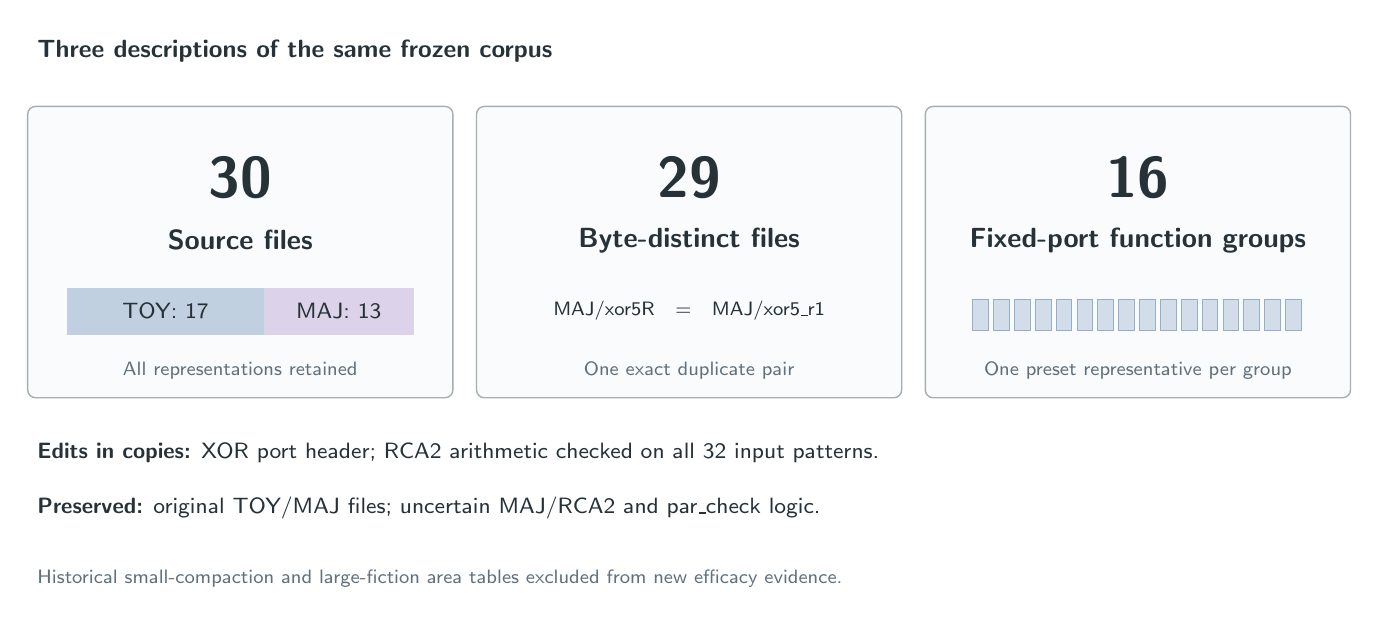
\begin{tikzpicture}[x=1mm,y=1mm]
\path[use as bounding box] (0,0) rectangle (168,74);
\node[paneltitle] at (0,71) {Three descriptions of the same frozen corpus};
\foreach \xx in {0,57,114}{\path[draw=ink!40,fill=grid!16,rounded corners=1mm,line width=.5pt] (\xx,27) rectangle (\xx+54,64);}
\node[font=\sffamily\bfseries\fontsize{20}{22}\selectfont] at (27,55) {30};
\node[font=\sffamily\bfseries] at (27,47) {Source files};
\path[fill=normal!35] (5,35) rectangle (30,41);
\path[fill=june!30] (30,35) rectangle (49,41);
\node at (17.5,38) {TOY: 17};\node at (39.5,38) {MAJ: 13};
\node[smallnote,anchor=center] at (27,30.5) {All representations retained};
\node[font=\sffamily\bfseries\fontsize{20}{22}\selectfont] at (84,55) {29};
\node[font=\sffamily\bfseries] at (84,47) {Byte-distinct files};
\node[align=center,font=\sffamily\fontsize{7.5}{9}\selectfont] at (84,38) {MAJ/xor5R\quad =\quad MAJ/xor5\_r1};
\node[smallnote,anchor=center] at (84,30.5) {One exact duplicate pair};
\node[font=\sffamily\bfseries\fontsize{20}{22}\selectfont] at (141,55) {16};
\node[font=\sffamily\bfseries] at (141,47) {Fixed-port function groups};
\foreach \k in {0,...,15}{\pgfmathsetmacro{\gx}{120+2.65*\k}\path[draw=normal!60,fill=normal!25,line width=.25pt] (\gx,35.5) rectangle (\gx+2,39.5);}
\node[smallnote,anchor=center] at (141,30.5) {One preset representative per group};
\node[anchor=west] at (0,20) {\textbf{Edits in copies:} XOR port header; RCA2 arithmetic checked on all 32 input patterns.};
\node[anchor=west] at (0,13) {\textbf{Preserved:} original TOY/MAJ files; uncertain MAJ/RCA2 and par\_check logic.};
\node[anchor=west,smallnote] at (0,4) {Historical small-compaction and large-fiction area tables excluded from new efficacy evidence.};
\end{tikzpicture}
\end{document}
